\documentclass[a4paper, singlepage, 11pt]{tubsreprt}
\usepackage[ngerman]{babel}
\usepackage[utf8]{inputenc}
\usepackage{cite}
\usepackage{graphicx}
\usepackage{wrapfig}
\title{Wärmebehandlung}
\date{Wintersemester 17/18}
\author{J. Hansen, S. Vodde,
 J. Veer, T. Stein}

\logo{
	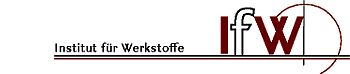
\includegraphics{Bilder/ifw-logo.jpg}
}

\begin{document}
\maketitle
\tableofcontents
\chapter{Titanwerkstoffe}

\section{Gefügemerkmale}
Wie andere Metalle liegt Titan in verschiedenen Gittermodifikationen beziehungsweise Phasenzuständen vor. Der Zustand ist von der Temperatur und den vorliegenden Legierungselementen abhängig. Bei reinem Titan liegt zwischen 1668°C und 882°C ein kubisch raumzentriertes Kristallgitter vor. Diese Phase wird als Betaphase ($\beta$-Phase) bezeichnet. Bei 882°C erfährt Titan eine Phasenumwandlung zu einem Hexagonalen Gitter. Die Phasenumwandlungstemperatur wird als Betatransus Temperatur bezeichnet. Sie ist für jede Legierung unterschiedlich, da Legierungselemente Einfluss auf diese haben \cite{Luetjering2007}.

Das hexagonale Gitter wird als Alphaphase ($\alpha$-Phase) bezeichnet. Daraus folgend ist reines Titan bei Raumtemperatur nahezu vollständig als Alphaphase vorliegend, sollte das Material langsam abgekühlt sein. 

Das hexagonale Gitter der Alphaphase ist annähernd dichtest gepackt. Das Verhältnis in der Zelle ist etwas kleiner als das in der dichtest gepackten Zelle. c:a von $\alpha$-Titan liegt bei 1.586. Die perfekte hexagonale Zelle hat ein Verhältnis von 1.624 \cite{Siemers2017}. c und a sind Längen innerhalb einer Zelle. Je nach Aufbau der Zelle sind diese Längen unterschiedlich groß.


\subsection{Alpha}
Die alpha-Titan Phase ist durch eine hexagonale Gitterstruktur gekennzeichnet. Dadurch entsteht ein anisotropes Werkstoffverhalten in einem Korn beziehungsweise Einkristall.
Ein Einkristall ist über ein homogenes, einhaltliches Kristallgitter definiert.
In einem Belastungsfall dieses Einkristalls ist das Werkstoffverhalten abhängig von der Belastungsrichtung, im Verhältnis zur Gitterrichtung. Das Elastizitätsmodul $E$ reicht je nach Verhältnis, von minimal 100 GPa bis maximal 145 GPa. Es ist eine Kenngröße, die das elastische Verhalten eines Werkstoffes definiert und wird in Pascal angegeben. 

Titan wird jedoch sehr selten als Einkristall hergestellt, sodass die unterschiedliche Kornorientierung dafür sorgt, das die anisotropie der einzelnen Körner sich gegenseitig aufhebt. Man kann somit von einem isotropen Werkstoffverhalten ausgehen.

Der $\beta$-$\alpha$ Umklappvorgang kann auch martensitisch erfolgen. Dafür werden Abkühlgeschwindigkeiten von mindestens 500 K/s benötigt. Ein resultierender Martensit ist aber nicht zwangsläufig mit einer Festigkeitssteigerung verbunden, da es nicht, wie beispielsweise im Martensit des Eisens, zu einer Gitterverzerrung kommt \cite[vgl. ]{Siemers2017}.
\subsection{Beta}
Eine $\beta$-Phase ist ein Gefüge mit einer kubisch raumzentrierten Gitteranordnung. Dadurch resultiert ein homogenes Werkstoffverhalten.

Das E-Modul und die Festigkeit der Betaphase ist deutlich geringer als die der Alphaphase. Das E-Modul der Betaphase erreicht

Eine große menge an $\beta$-Phase existiert in der Regel bei Raumtemperatur nur unter bestimmten Bedingungen. Sie kann als metastabile Phase auftreten. Dies bedeutet, dass das Material nicht vollständig den Phasenübergang abschließen konnte und so in dem Zustand aus höheren Temperaturen verblieben ist. 

Durch Zusatz bestimmter Legierungselemente kann sie auch in größeren Mengen vorliegen. Dies wird im Kapitel betastabilisierende Legierungselemente näher erläutert.
\subsection{Gefüge}
Da sich die Arbeit vor allem mit Gefügeausprägungen und ihren Auswirkungen auseinandersetzt, werden die grundlegenden hier vorgestellt. Die jeweiligen Ausprägungen sind Ausschlaggebend wie sich das Material mechanisch verhält. Da die mögliche Wärmebehandlung nach dem Rekristallisieren statt findet, sind einige Gefügeausbildungen möglicherweise nicht möglich. Dies ist abhängig von dem Ausgangsgefüge.
Es sind auch Kombinationen der einzelnen Gefüge möglich, um Vorteile der einzelnen hinsichtlich ihrer mechanischen Eigenschaften zu kombinieren.
\subsubsection{Lamellar}
In Abbildung 1.1 ist ein Volllamellares Gefüge zu sehen. Es Kennzeichnet sich durch fein parallel verlaufende Nadeln. Die breite der einzelnen Nadeln hängt mit der Abkühlgeschwindigkeit zusammen. In dieser Abbildung wurde eine schnelle Abkühlung gewählt, was zu kleinen, feinen Nadeln führt. 

Lamellare Gefüge entstehen aus einer Abkühlung aus dem $\beta$-Gebiet. Während des Abkühlens bilden sich in den Korngrenzen der $\beta$-Phase $\alpha$-Bereiche, die in das $\beta$-Korn hinein wachsen. Die Alphabereiche wachsen erst in eine Richtung bevor sie ihre Dicke erhöhen. Je nach Abkühlgeschwindigkeit entstehen so dünne oder dickere Nadeln. Das Bild zeigt ein beispielhaftes Gefüge, indem voll lamellare Strukturen zu sehen sind. Diese sind in diesem Beispiel martensitisch. 

\begin{minipage}{\textwidth}


	\centering
		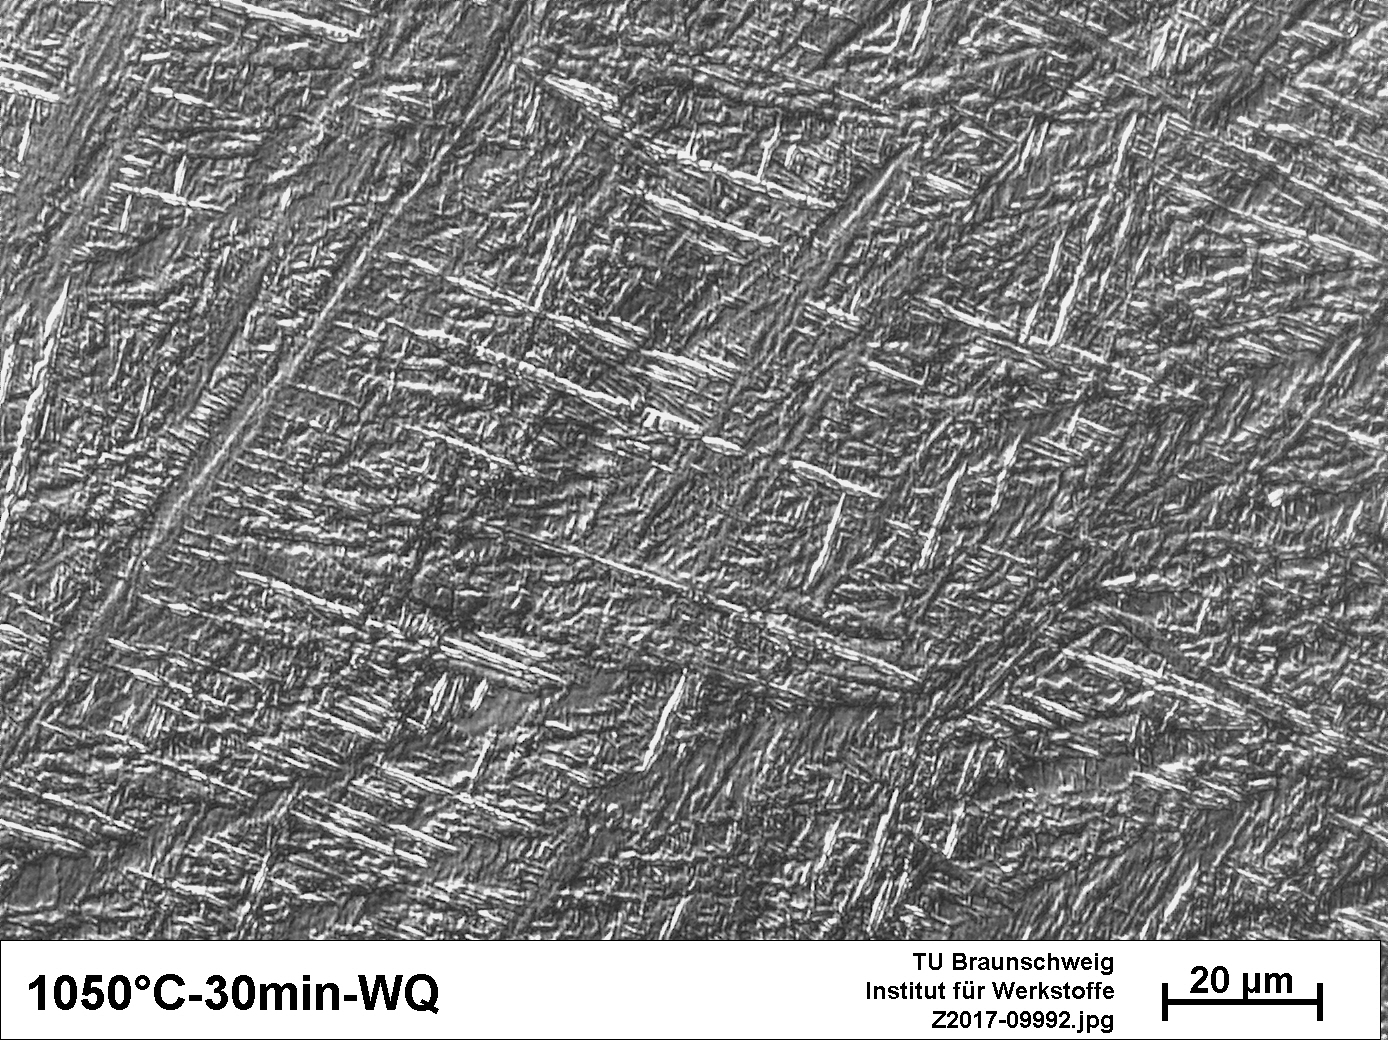
\includegraphics[scale=0.5]{Bilder/Vollmartensit.jpg}
		\captionof{figure}{Volllamellares Gefüge}
		\label{fig1}
		
\end{minipage}

\subsubsection{Bimodal}
\subsubsection{Globular}
\chapter{Methodik}
\section{Wärmebehandlung}

Die Wärmebehandlung nach der Rekristllisation ist die letzte Methode um das Gefüge des Titans einzustellen. Hierbei kommt es auf Parameter wie Temperatur, Haltezeit und Abkühlmethode an. Um die bereits erwähnten Gefüge zu realisieren, ist eine spezifische Abfolge von einer beziehungsweise mehreren Stufen einer Wärmebehandlung nötig. Die grundlegenden Behandlungen werden in diesem Kapitel behandelt. Spezielle, mehrstufige Behandlungen werden in dem dritten Kapitel behandelt.
\paragraph{Temperaturkontrolle}
Für die Temperaturkontrolle innerhalb der Wärmebehandlung kommt ein Ofen zum Einsatz. Dieser kann bis Temperaturen weit über Betatransus aufheizen und diese, mit einer Genauigkeit von drei Kelvin, halten. 

Der Ofen ist außerdem für die Aufheizgeschwindigkeit verantwortlich, da diese auch einen wichtigen Einfluss haben kann.
\paragraph{Abkühlmedien}

Durch Abkühlmedien werden bestimmte Abkühlgeschwindigkeiten realisiert. Für langsamere Abkühlungen als in der Luft wird der Ofen genutzt. Hier kann die Temperatur beliebig langsam reduziert werden. Ein weiterer Vorteil des Ofens ist, dass die Probe auf eine bestimmte Temperatur herunter gekühlt werden kann. Dies ist für mehrstufige Wärmebehandlungen wichtig, bei denen eine Abkühlung auf Raumtemperatur zwischen den Schritten vermieden werden soll. 

Da der Ofen nicht überaus schnell abkühlen kann, wird zur schnelleren Abkühlung Luft mit Raumtempertur verwendet. Durch den höheren Temperaturgradienten im Verhältnis zum Ofen wird so die Abkühlung beschleunigt.  

Um noch schnellere Abkühlungen zu realisieren wird Wasser oder Öl verwendet. So werden zum Beispiel Abkühlgeschwindigkeiten für eine Martensitbildung ermöglicht. Gleichzeitig wird das Gefüge aus dem Hochtemperaturbereich "eingefroren." Die Phasen liegen somit metastabil auf Raumtemperaturniveau vor. Metastabil bedeutet das die Phase unter normalen Umständen nicht vorliegt. Die Phasenumwandlungen sind nicht möglich da die Diffusionsgeschwindigkeiten bei Raumtemperatur gering sind, beziehungsweise eine Diffusion nicht statt findet. Gleichzeitig ist die Abkühlgeschwindigkeit so groß, dass 
\subsection*{Anpassung der Gefüge durch Wärmebehandlung}

Das Anpassen der Gefüge ist das Ziel der Wärmebehandlungen. So werden Werkstoffeigenschaften gezielt für den jeweiligen Anwendungsfall optimiert. Bestimmte Gefüge folgen aus bestimmten Wärmebehandlungen.
\bibliographystyle{plain}
\bibliography{literatur}

\end{document}
